\documentclass[a4paper, english, 12pt]{article} % norsk & english is supported

\newcommand{\exerciseNumber}{5}
\newcommand{\solutions}{false} % Change to   true   to create solutions
% Must be defined before course package, \exerciseNumber, and \solutions
\usepackage{IMF}

\usepackage{MA0301}

\begin{document}

\titlebox

\begin{problem}[2]
  Let $Y := \{ 1,2,3,4,\ldots,600 \}$. Use the inclusion-exclusion principle to
  find the number of positive integers $Y$ that are not divisible by $3$, $5$ or $7$.
\end{problem}


\begin{answer}
  \begin{figure}[htbp!]
    \centering
    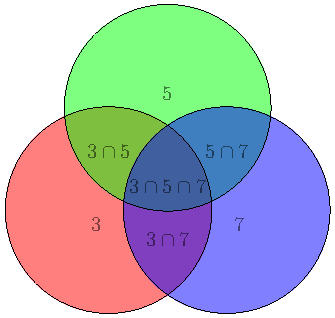
\includegraphics{Venn-Diagram-5}
    \caption{}
    \label{fig:venn}
  \end{figure}
  % 
  While not relevant for the exam, the Venn diagram displayed in \cref{fig:venn}
  can shed some light on why the inclusion-exclusion principle works. We are
  interested in finding cardinality\footnote{In mathematics, the cardinality of
    a set $A$ is a measure of the ''number of elements of the set``, $|A|$.} of the union
  $3 \cup 5 \cup 7$, where the numbers are now interpreted as sets e.g. $3 =
  \{3n \mid n \in Y\}$ is the subset of $Y$ consisting of all numbers divisible
  by 3 and so forth. The following argument might be a bit hard to digest, so
  try to read it while carefully studying \cref{fig:venn}.

  Simply adding the number of elements in each set will give us an
  over-estimate. As an example $15$ is counted twice, once in the set with
  numbers divisible by 3, and once in the set consisting of numbers divisible by
  $5$. Thus $|3 \cup 5 \cup 7| \neq |3| + |5|+|7|$. To remedy this we can remove
  every union of two integers: $|3 \cap 5| + |3 \cap 7| + |3 \cap 7|$. However,
  this creates another problem. Take $105 = 3 \cdot 5 \cdot 7$. This number is
  included three times as it lies in $3$, $5$ and $7$, alas it is also removed
  three times since it lies in $3 \cap 5$, $3 \cap 7$ and $5 \cap 7$. Thus, we
  need to include back every number that is a multiple of $3$, $5$ and $7$. This
  gives us our final expression,
  %
  \begin{equation*}
    |3 \cup 5 \cup 7| = |3| + |5| + |7| - |3 \cap 5| - |3 \cap 7| - |5 \cap 7| + |3 \cap 5 \cap 7|,
  \end{equation*}
  %
  which is precisely the inclusion-exclusion principle.
  %
  The number of integers that are a multiple of $k$ beneath $n$ are precisely
  $\lfloor {n/k} \rfloor$. Every number divisible by $3$, $5$ or $7$ is thus
  %
  \begin{align*}
        |3 \cup 5 \cup 7|
    & = |3| + |5| + |7| - |3 \cap 5| - |3 \cap 7| - |5 \cap 7| + |3 \cap 5 \cap 7| \\
    & = \lfloor \frac{600}{3} \rfloor
    +   \lfloor \frac{600}{5}  \rfloor
    +  \lfloor \frac{600}{7}  \rfloor  
    -  \lfloor \frac{600}{3\cdot 5}  \rfloor
    -  \lfloor \frac{600}{3\cdot 7}  \rfloor 
    -  \lfloor \frac{600}{5 \cdot 7}  \rfloor
      +  \lfloor \frac{600}{3\cdot 5\cdot 7} \rfloor  \\
    & = 200 + 120 + 85 - 40 - 28 - 17 + 5 
      = 325\,.
  \end{align*}
  %
  As such, there are $|Y| - |3 \cup 5 \cup 7| = 275$ numbers not divisible by $3$,
  $5$ or $7$ amongst the first $600$ integers.
\end{answer}

\begin{problem}
  Use the principle of induction to show that for all natural numbers $n$,
  \begin{equation*}
    4 \sum_{i=1}^n i(i+2)(i+4) = n(n+1)(n+4)(n+5).
  \end{equation*}
\end{problem}

\begin{answer}
  \paragraph{Base case:} For $n=1$
  %
  \begin{align*}
    LHS = 4 \sum_{i=1}^{1} i(i+2)(i+4) = 4\cdot 1 \cdot 3 \cdot 5 = 60\,,
    && RHS = 1(1+1)(1+4)(1+5) = 60\,,
  \end{align*}
  %
  so the hypothesis holds for the base case.
  \paragraph{inductive step:} Assume that for all $k$ we have
  %
  \begin{equation*}
    4 \sum_{i=1}^k i(i+2)(i+4) = k(k+1)(k+4)(k+5).
  \end{equation*}
  %
  We wish to prove that this implies that the hypothesis holds for $k+1$.
  %
  \begin{align*}
    RHS & = (k+1)(k+2)(k+5)(k+6) \\
    LHS & = 4 \sum_{i = 1}^{k+1} i(i+2)(i+4) \\
        & = 4 (k+1)(k+3)(k+5) + 4 \sum_{i=1}^{k} i(i+2)(i+4) \\
        & = 4 \textcolor{gray}{(k+1)}(k+3)\textcolor{gray}{(k+5)} + k\textcolor{gray}{(k+1)}(k+4)\textcolor{gray}{(k+5)} \\
        & = [4(k+3) + k(k+4)]\textcolor{gray}{(k+1)(k+5)} \\
        & = (k+1)(k+2)(k+5)(k+6).
  \end{align*}
  %
  As $LHS = RHS$ the rest follows by induction. The steps performed in the
  calculation above where respectively: (1)
  %
  \begin{equation*}
    \sum_{i=1}^{n+1} a_i = a_1 + a_2 + \cdots + a_{n} + a_{n+1}
    = ( a_1 + a_2 + \cdots a_{n} ) + a_{n+1}
    = a_{n+1} + \sum_{i = 1}^{n} a_i.
  \end{equation*}
  %
  (2) use the induction hypothesis. (3) We
  have $4(k+3) + k(k+4) = k^2 + 8k + 12 = (k+6)(k+2)$ either by the quadratic
  formula, or inspection (as $6+2 = 8$ and $6\cdot 2 = 12$).
\end{answer}
  

\begin{problem}[7]
  Use the laws of set theory to show for arbitrary sets $A$, $B$, $C$ that:
\end{problem}

\begin{subproblem}
  If $(A \cup B) \subseteq (A \cap B)$ then $A = B$.
\end{subproblem}

\begin{answer}
  To prove that $A = B$ we show that $A \subseteq
  B$ and $B \subseteq A$ when the conditions holds
  %
  \begin{align*}
    & A \subseteq A \cup B \subseteq A \cap B \subseteq B  \\
    & B \subseteq A \cup B \subseteq A \cap B \subseteq A,
  \end{align*}
  %
  and we are done.
\end{answer}

\begin{subproblem}
  $\overline{A \cap B} = \overline{A} \cup \overline{B}$.
\end{subproblem}

\begin{answer}
  So we are to prove De Morgan's first law, which suddenly is different in set
  notation compared to logic... Again we prove both inclusions.
  \begin{enumerate}[align=left]
    \item[$ \overline{A \cap B} \subseteq \overline{A} \cup \overline{B}$:]
   Assume that $x \in \overline{A \cap B}$. Then $x \neq A \cap B$, so either
   $x\not \in A$ or $x \not \in B$. Which, is the same as to say that $x
  \in \overline{A}$ or $x \in \overline{B}$. In either case $x \in \overline{A}
  \cup \overline{B}$.
  \item[$\overline{A} \cup \overline{B} \subseteq \overline{A \cap B}$:]
    Let $x \in \overline{A} \cup \overline{B}$. Then we know that either $x \not
    \in A$ or $x \not \in B$. Then it is not in the intersection either $x \not
      \in A \cap B$, which is to say $x \in \overline{A \cap B}$ and we are done.
      \end{enumerate}
\end{answer}

\begin{subproblem}
  $A \cap (B \cup C) = (A \cap B) \cup (A \cap C)$.
\end{subproblem}

\begin{answer}
  As before we prove both inclusions
  %
  \begin{enumerate}[align=left]
    \item[$A \cap (B \cup C) \subseteq (A \cap B) \cup (A \cap C)$:] Assume that
      $x \in A \cap (B \cup C)$. This implies that $x \in A$ and $x \in B \cup
      C$. The last expression is the same as saying that $x \in B$ or $x \in C$.
      If $x \in B$ then $x \in A \cap B$ (as $x \in A$), otherwise if $x \in C$ then $x \in A
      \cap C$. As $x$ is in either of those we at least have $x$ in the union $x
      \in (A \cap B) \cup (A \cap C)$.
      %
    \item[$(A \cap B) \cup (A \cap C) \subseteq A \cap (B \cup C)$:]
      Assume now that $x \in (A \cap B) \cup (A \cap C)$, as such $x \in (A \cap
      B)$ or $x \in (A \cap C)$. In the first case $x \in A$ and $x \in B$, in
      the latter $x \in A$ and $x \in C$. Regardless, $x \in A$. This leaves us
      with two cases either $x \in B$ or $x \in C$. In either case, $x$ has to
      lie in the union $x \in B \cup C$. This proves the inclusion
      $(A \cap B) \cup (A \cap C) \subseteq A \cap (B \cup C)$ and we are
      done.  
  \end{enumerate} 
\end{answer}


\ifthenelse{\boolean{\solutions}}{\newpage}{}

\seksjon{4.1}

\begin{problem}
  Prove each of the following for all $n \geq 1$ by the Principle of
  Mathematical induction
\end{problem}

\begin{subproblem}
  $\displaystyle 1^2 + 3^2 + 5^2 + \cdots + (2n-1)^2 = \frac{n(2n-1)(2n+1)}{3}$.
\end{subproblem}

\begin{answer}
  \paragraph{Base case:} For $n=1$ we have
  %
  \begin{equation*}
    LHS = (2\cdot 1 - 1)^2 = 1\,, \qquad
    RHS = \frac{1(2\cdot 1 - 1) (2\cdot 1 + 1)}{3} = \frac{1 \cdot 1 \cdot 3}{3} = 1,
  \end{equation*}
  %
  so the hypothesis holds for the base case.

  \paragraph{Inductive step:} Assume that the statement holds for $n=k$, in
  other words
  %
  \begin{equation*}
    \sum_{i=1}^n (2i-1)^2 = \frac{n(2n-1)(2n+1)}{3}.
  \end{equation*}
  %
  Need to show that this implies that the statement holds for $n=k+1$
  %
  \begin{align*}
    RHS & = \frac{(k+1)(2k+1)(2k+3)}{3} \\
    LHS & = \sum_{i=1}^{k+1} (2i-1)^2 \\
        & = (2k+1)^2 + \sum_{i=1}^k (2i-1)^2 \\
        & = (2k+1)^2 + \frac{k(2k-1)(2k+1)}{3} \\
        & = \frac{(2k+1)[3(2k+1) + k(2k-1)])}{3} \\
        & = \frac{(k+1)(2k+1)(2k+3)}{3}\,.
  \end{align*}
  %
  As $3(2k+1) + k(2k-1) = 2k^2 + 5k + 3 = (k+1)(2k+3)$ either by inspection or
  the quadratic formula. The rest follows now by induction, and thus concludes
  the proof.
\end{answer}

\begin{subproblem}
  $\displaystyle 1 \cdot 3 + 2 \cdot 4 + 3 \cdot 5 + \cdots + n(n+2) = \frac{n(n+1)(2n+7)}{6}$.
\end{subproblem}

\begin{answer}
  \paragraph{Base case:} For $n = 1$ we have,
  %
    \begin{equation*}
    LHS = 1 \cdot (2\cdot 1 + 1) = 3\,, \qquad
    RHS = \frac{1 (1 + 1)(2\cdot 1 + 7)}{6} = \frac{1 \cdot 2 \cdot 9}{6} = 3,
  \end{equation*}
  %
  so the hypothesis holds for the base case.

  \paragraph{Inductive step:} Assume that the statement holds for $n = k$, that
  is
  %
  \begin{align*}
    \sum_{i=1}^k i(i+2) = \frac{k(k+1)(2k+7)}{6}.
  \end{align*}
  %
  Wish to show that this implies that the statement holds for $n=k+1$.
  %
  \begin{align*}
    RHS & = \frac{(k+1)(k+2)(2k+9)}{6} \\
    LHS & = \sum_{i=1}^{k+1} i(i+2)   \\
        & = (k+1)(k+3) + \sum_{i=1}^{k} i(i+2)  \\
        & = (k+1)(k+3) + \frac{k(k+1)(2k+7)}{6} \\
        & = \frac{(k+1)[(6(k+3) + k(2k+7))]}{6} \\
        & = \frac{(k+1)(k+2)(2k+9)}{6}.
  \end{align*}
  %
  As $6(k+3) + k(2k+7) = 2k^2 + 13k + 18 = (k+2)(2k+9)$ either by inspection or
  the quadratic formula. The rest follows now by induction, and thus concludes
  the proof.
\end{answer}

\begin{subproblem}
  $\displaystyle \sum_{i = 1}^n \frac{1}{i(i+1)} = \frac{n}{n+1}$.
\end{subproblem}

\begin{answer}
  While the question \emph{clearly} states that the proof has to be done by
  induction, I can not help myself to show the following proof as the series is
  telescoping
  %
  \begin{equation*}
    \sum_{i = 1}^n \frac{1}{i(i+1)}
    = \sum_{i=1}^n \frac{1}{i} - \frac{1}{i+1}
    = \frac{1}{1} - \frac{1}{2} + \frac{1}{2} - \frac{1}{3} + \cdots
    + \frac{1}{n} - \frac{1}{n+1}
    = 1 - \frac{1}{n+1} = \frac{n}{n+1}.
  \end{equation*}
  %
  \paragraph{Base case:} For $n=1$ we have
  %
  \begin{equation*}
    LHS = \sum_{i=1}^1 \frac{1}{i(i+1)} = \frac{1}{1(1+1)} = \frac{1}{2}\,, \qquad
    RHS = \frac{1}{1+1} = \frac{1}{2},
  \end{equation*}
  %
  so the hypothesis holds for the base case.
  \paragraph{Inductive step:} Assume that the statement holds for $n=k$, that is
  %
  \begin{equation*}
    \sum_{i = 1}^k \frac{1}{i(i+1)} = \frac{k}{k+1}
  \end{equation*}
  %
  Wish to show that this implies that the statement holds for $n=k+1$
  %
  \begin{align*}
    RHS & = \frac{k+1}{k+2} \\
    LHS & = \sum_{i = 1}^{k+1} \frac{1}{i(i+1)} \\
        & = \frac{1}{(k+1)(k+2)} + \sum_{i=1}^{k} \frac{1}{k(k+1)} \\
        & = \frac{1}{(k+1)(k+2)} + \frac{k}{k+1} \\
        & = \frac{1 + k(k+2)}{(k+2)(k+1)} 
          = \frac{(1+k)^2}{(k+2)(k+1)} = \frac{1+k}{k+2}
  \end{align*}
  %
  As $1 + k(k+2) = k^2 + 2k + 1^2 = (k+1)^2$ either by inspection or
  the quadratic formula. The rest follows now by induction, and thus concludes
  the proof.
\end{answer}


\begin{problem}[12]
  \begin{subproblem}
    \label{subproblem:12a}
    Prove that $(\cos \theta + i \sin \theta)^2 = \cos 2\theta + i \sin
    2\theta$ where $i \in \C$ and $i^2 = -1$.
  \end{subproblem}
\end{problem}

\begin{answer}
  By De Moivre's laws we have
  %
  \begin{align*}
    (\cos \theta + i \sin \theta)^2
    = (e^{i \theta})^2
    = e^{i 2 \theta}
    = \cos 2 \theta + i \sin \theta
  \end{align*}
  %
  However, this might be considered cheating as we are supposed to prove this
  theorem later. Expanding the square gives the same results
  %
  \begin{align*}
    (\cos \theta + i \sin \theta)^2
    & = \cos^2 \theta + 2 i \cos \theta \sin \theta + i^2 \sin^2 \theta \\
    & = (\cos^2 \theta - \sin^2 \theta) + i (2 \cos \theta \sin \theta)
    = \cos (2 \theta) + i \sin (2 \theta)
  \end{align*}
\end{answer}

\begin{subproblem}
  Using induction, prove that for all $n \in \Z^+$,
  %
  \begin{equation*}
    (\cos \theta + i \sin \theta)^n = \cos n\theta + i \sin n\theta,
  \end{equation*}
  %
\end{subproblem}

\begin{answer}
  \paragraph{Base case:} As $n \in \Z^+$, the base case is $n=0$,
  %
  \begin{equation*}
    RHS = (\cos \theta + i \sin \theta)^0 = 1\,, \qquad
    LHS = \cos (0\cdot \theta) + i \sin (0\cdot \theta) = 1.
  \end{equation*}
  %
  as $\cos 0 = 1$ and $\sin 0 = 0$ so the hypothesis holds for the base case.
  (\Cref{subproblem:12a} shows that the hypothesis holds for $n=1$ as well.)

  \paragraph{Inductive step:} Assume that the statement holds for $n=k$ that is
  \begin{equation*}
    (\cos \theta + i \sin \theta)^k = \cos k\theta + i \sin k\theta,
  \end{equation*}
  %
  want to prove that this implies that the statement holds for $n=k+1$. Now
  %
  \begin{align*}
    RHS & = \cos (k+1)\theta + i \sin (k+1) \theta \\
    LHS & = (\cos \theta + i \sin \theta)^{k} (\cos \theta + i \sin \theta) \\
        & = (\cos k \theta + i \sin k \theta) (\cos \theta + i \sin \theta) \\
        & = (\cos \theta \cos k \theta - \sin \theta \sin k \theta )+
          i (\sin k \theta \cos \theta + \sin \theta \cos k \theta ) \\
        & = \cos(k+1)\theta + i \sin(k+1) \theta
  \end{align*}
  %
  since $RHS=LHS$ the statement follows by induction.
\end{answer}

\begin{subproblem}
  Verify that $1 + i = \sqrt{2}(\cos 45^\circ + i \sin 45^\circ)$, and compute $(1+i)^{100}$.
\end{subproblem}

\begin{answer}
  As $\cos \pi/4 = \sin \pi/4 = 1/\sqrt{2}$, the first part is trivial
  %
  \begin{equation*}
    \sqrt{2}( \cos \pi/4 + i \sin \pi/4) = \sqrt{2}\left( \frac{1}{\sqrt{2}} + i \frac{1}{\sqrt{2}} \right) = 1 + i
  \end{equation*}
  %
  and so $(1+i)^{100} = (\sqrt{2})^{100}(\cos \pi/4 + i\sin \pi/4)^{100} =
  2^{50}(\cos 25 \pi + i \sin 25 \pi) = -2^{50}$
\end{answer}

\begin{problem}[16]
  \begin{subproblem}
    \label{subprob:16a}
    For $n=3$ let $X_3 = {1,2,3}$. Now consider the sum
    %
    \begin{equation*}
      s_3 = \frac{1}{1} + \frac{1}{2} + \frac{1}{3}
      + \frac{1}{1\cdot 2} + \frac{1}{ 1 \cdot 3} + \frac{1}{2 \cdot 3} + \frac{1}{1 \cdot 2 \cdot 3} \\
       = \sum_{\emptyset \neq A \subseteq X_3} \frac{1}{p_A},
     \end{equation*}
     %
     where $p_A$ denotes the product of all elements in a non-empty subset $A$
     of $X_3$. Note that the sum is taken over all the non-empty subsets of
     $X_3$. Evaluate this sum
  \end{subproblem}
\end{problem}

\begin{answer}
  Finding the common denominator a straight forward computation yields
  \begin{align*}
      s_3 & = \frac{1}{1} + \frac{1}{2} + \frac{1}{3}
    + \frac{1}{1\cdot 2} + \frac{1}{ 1 \cdot 3} + \frac{1}{2 \cdot 3} + \frac{1}{1 \cdot 2 \cdot 3} \\
          & = \left(   \frac{1}{1} + \frac{1}{2} + \frac{1}{1 \cdot 2} \right)
            + \left(  \frac{1}{3} + \frac{1}{1\cdot 3} + \frac{1}{2 \cdot 3} + \frac{1}{1 \cdot 2 \cdot 3} \right)\\
          & = \left(   \textcolor{gray}{\frac{1}{1} + \frac{1}{2} + \frac{1}{1 \cdot 2}} \right)
            + \left( 1 + \textcolor{gray}{\frac{1}{1} + \frac{1}{2} + \frac{1}{1 \cdot 2}} \right)\frac{1}{3}
            = \textcolor{gray}{2} + (1 + \textcolor{gray}{2})\frac{1}{3} = 3
  \end{align*}
\end{answer}

\begin{subproblem}
    \label{subprob:16b}
  Repeat the calculation in \cref{subprob:16a} for $s_2$ and $s_4$.
\end{subproblem}

\begin{answer}
  By ``accident'' $s_2$ has already been computed
  %
  \begin{align*}
    s_2 = \frac{1}{1} + \frac{1}{2} + \frac{1}{1 \cdot 2} = 1 + \frac{1}{2} + \frac{1}{2} = 2
  \end{align*}
  %
  $s_4$ is done in the same matter, albeit a bit more work has to be done
  %
  \begin{align*}
        s_4
    & = \frac{1}{1} + \frac{1}{2} + \frac{1}{3} + \frac{1}{4}
      + \frac{1}{1 \cdot 2} + \frac{1}{1 \cdot 3} + \frac{1}{1 \cdot 4} 
      + \frac{1}{2 \cdot 3} + \frac{1}{2 \cdot 4} + \frac{1}{3 \cdot 4} \\
    & + \frac{1}{1 \cdot 2 \cdot 3} + \frac{1}{1 \cdot 2 \cdot 4} + \frac{1}{1 \cdot 3 \cdot 4}
    + \frac{1}{2 \cdot 3 \cdot 4} + \frac{1}{1\cdot 2 \cdot 3 \cdot 4} \\
    & = \left(   \frac{1}{1} + \frac{1}{2} + \frac{1}{3}
      + \frac{1}{1\cdot 2} + \frac{1}{ 1 \cdot 3} + \frac{1}{2 \cdot 3} + \frac{1}{1 \cdot 2 \cdot 3} \right)\\
    & + \left[ \frac{1}{4}
      + \frac{1}{1\cdot 4} + \frac{1}{2 \cdot 4} + \frac{1}{3 \cdot 4} + \frac{1}{2 \cdot 3 \cdot 4} + \frac{1}{1 \cdot 3 \cdot 4} + \frac{1}{1 \cdot 2 \cdot 4} + \frac{1}{1 \cdot 2 \cdot 3 \cdot 4}\right] \\
    & = \left(   \textcolor{gray}{\frac{1}{1} + \frac{1}{2} + \frac{1}{3}
      + \frac{1}{1\cdot 2} + \frac{1}{ 1 \cdot 3} + \frac{1}{2 \cdot 3} + \frac{1}{1 \cdot 2 \cdot 3}} \right)\\
    & + \left[ 1 
      +  \left( \textcolor{gray}{\frac{1}{1} +  \frac{1}{2} + \frac{1}{3} + \frac{1}{2 \cdot 3} + \frac{1}{1 \cdot 3} + \frac{1}{1 \cdot 2} + \frac{1}{1 \cdot 2 \cdot 3}}\right)\right] \cdot \frac{1}{4} \\
    & = \textcolor{gray}{s_3} + [1 + \textcolor{gray}{s_3}]\frac{1}{4} = 3 + (1+3)\frac{1}{4} = 4 
  \end{align*}
\end{answer}

\begin{subproblem}
  Conjecture a general result suggested by the calculations from
  \cref{subprob:16a,subprob:16b}. Prove your conjecture using the Principle of
  Mathematical induction.
\end{subproblem}

\begin{answer}
  \noindent
  Interesting problem! I conjecture that for every $n \in \N$, $s_n = n$.
  \paragraph{Base case:} As $n \in \N$ the base case is $n = 1$. Then,
  %
  \begin{equation*}
    LHS = s_1 = \frac{1}{1} = 1 \,, \qquad
    RHS = 1,
  \end{equation*}
  %
  and so the hypothesis holds for the base case.
  
  \paragraph{Inductive step:} We assume that for every $k$ we have
  %
  \begin{equation*}
    s_k = \sum_{\emptyset \neq A \subset X_k} \frac{1}{p_A} 
  \end{equation*}
  %
  wish to prove that this implies that the conjecture holds for $s_{k+1}$, then
  %
  \begin{equation}
    \label{eq:subsetsum}
    s_{k+1}
      = \sum_{\emptyset \neq A \subset X_{k+1}} \frac{1}{p_A}
      = \sum_{\emptyset \neq A \subset X_{k}} \frac{1}{p_B}
      + \sum_{\{k+1\} \subseteq A \subset X_{k+1}} \frac{1}{p_C}\\ 
  \end{equation}
  %
  Where the first sum is taken over all non-empty subsets $B$ of $X_k$ and the
  second sum over all subsets $C$ of $X_{k+1}$ that contain $k+1$. In other
  words, we do as before and isolate all the terms that contain $k+1$. As seen
  before we can factor out the $1/(k+1)$ term giving
  %
  \begin{equation*}
    s_{k+1}
    = s_k + \frac{1}{1+k} (1 + s_k) = k + \frac{1}{1+k}(1+k) = 1 + k
  \end{equation*}
  Why the second sum in \cref{eq:subsetsum} equals $(1+s_k)/(1+k)$ has been shown in excruciating
  detail in
  \cref{subprob:16a,subprob:16b}. The proof for the conjecture now follows by induction.
\end{answer}

% \ifthenelse{\boolean{\solutions}}{\newpage}{}

\begin{problem}
  For $n \in \Z^+$. We define the $n$'th harmonic number $H_n$ as the sum
  of the first $n$ reciprocals (of the natural integers),  $H_n = \sum_{i=1}^n 1/i$.
\end{problem}

\begin{subproblem}
  For all $n \in \N$ prove that $1 + \frac{n}{2} \leq H_{2^n}$.
\end{subproblem}

\begin{answer}
  \paragraph{Base case:} As $n \in \N$ the base case is $n=1$. Then
  %
  \begin{equation*}
    LHS = 1 + \frac{1}{2} \,, \qquad
    RHS = H_{2^{0+1}} = H_2 = 1 + \frac{1}{2}
  \end{equation*}
  %
  so the hypothesis holds for the base case.
  \paragraph{Inductive step:} Assume that the statements holds for $n=k$ that is
  %
  \begin{equation*}
    1 + \frac{n}{2} \leq H_{2^{n+1}}
  \end{equation*}
  %
  wish to show that this implies that the inequality holds for $n=k+1$. Then,
  %
  \begin{align*}
    LHS & = 1 + \frac{k+1}{2} \\
    RHS & = H_{2^{k+1}} \\
    & = H_{2^k} + \frac{1}{2^k+1} + \frac{1}{2^k + 2} + \cdots + \frac{1}{2^k + 2^k} \\
    & \geq H_{2^k} + \frac{1}{2^k+2^k} + \frac{1}{2^k + 2^k} + \cdots + \frac{1}{2^k + 2^k} \\
    & = H_{2^k} + \frac{2^k}{2 \cdot 2^k}
      = H_{2^{k}} + \frac{1}{2}
      \geq 1 + \frac{k}{2} + \frac{1}{2} = 1 + \frac{k+1}{2}
  \end{align*}
  %
  as $LHS = RHS$ the rest follows by induction. 
\end{answer}

\begin{subproblem}
  Prove that for all $n \in \Z^+$,
  %
  \begin{equation*}
    \sum_{j=1}^n j H_j
    = \left[ \frac{n(n+1)}{2} \right] H_{n+1} - \left[ \frac{n(n+1)}{4} \right].
  \end{equation*}
\end{subproblem}

\begin{answer}
  \paragraph{Base case:} As $n \in \Z^+$ the base case is $n=0$ then
  %
  \begin{equation*}
    RHS = \sum_{j=1}^{0} j H_j = 0, \qquad 
    LHS  
    = \left[ \frac{0 \cdot (0+1)}{2} \right] H_{0+1} - \left[ \frac{0 \cdot (0+1)}{4} \right] = 0,
  \end{equation*}
  %
  so the hypothesis holds for the base case.
  
  \paragraph{Inductive step:}Assume that
  %
  \begin{equation*}
    \sum_{j=1}^k j H_j
    = \left[ \frac{k(k+1)}{2} \right] H_{k+1} - \left[ \frac{k(k+1)}{4} \right]
  \end{equation*}
  % 
  holds for every $n = k$. Wish to prove that this implies that the statement
  holds for $n = k + 1$. Now
  %
  \begin{align*}
    LHS & = \left[ \frac{(k+1)(k+2)}{2} \right] H_{k+2} - \left[ \frac{(k+1)(k+2)}{4} \right]\\
    RHS & = \sum_{j=1}^{k+1} j H_j = (k+1) H_{k+1} + \sum_{j=1}^{k} j H_j \\
        & = (k+1)H_{k+1} + \left[ \frac{k(k+1)}{2} \right] H_{k+1} - \left[ \frac{k(k+1)}{4} \right] \\
        & \frac{(k+1)(k+2)}{2} H_{k+1} - \frac{k(k+1)}{4} \\
        & \frac{(k+1)(k+2)}{2} \left[ H_{k+2} - \frac{1}{k+2} \right] - \frac{k(k+1)}{4} \\
        & \frac{(k+1)(k+2)}{2} H_{k+2} - \frac{2(k+1)}{4} - \frac{k(k+1)}{4} \\
        & \frac{(k+1)(k+2)}{2} H_{k+1} - \frac{(k+1)(k+2)}{4}
  \end{align*}
  %
  As $LHS = RHS$ the proof follows by induction.
\end{answer}

\end{document}
